\section{Examples}
\showtoc

\subsection{Examples}

\begin{frame}
  \frametitle{Example: Compass Gait as a Shaped System}
  \only<1>{
    \begin{columns}
      \column{1.5in}
      Dynamic Model:
      \begin{align*}
        M(q) \ddot q + H(q, \dot q) = B(q) u
      \end{align*}
      Control Law:
      \begin{align*}
        \bar u(q) &= G(q) - G(\Psi(q))
      \end{align*}

      \column{1.5in}
      \begin{figure}
        \centering
        \def\svgwidth{1.0\columnwidth}
        \input{../figs/cg2d-2link-model.eps_latex}
        \vspace{-2em}
        \caption{Compass-gait biped with Controlled Symmetries.}
      \end{figure}
    \end{columns}
  }
  \only<2>{
    \begin{figure}
      \centering
      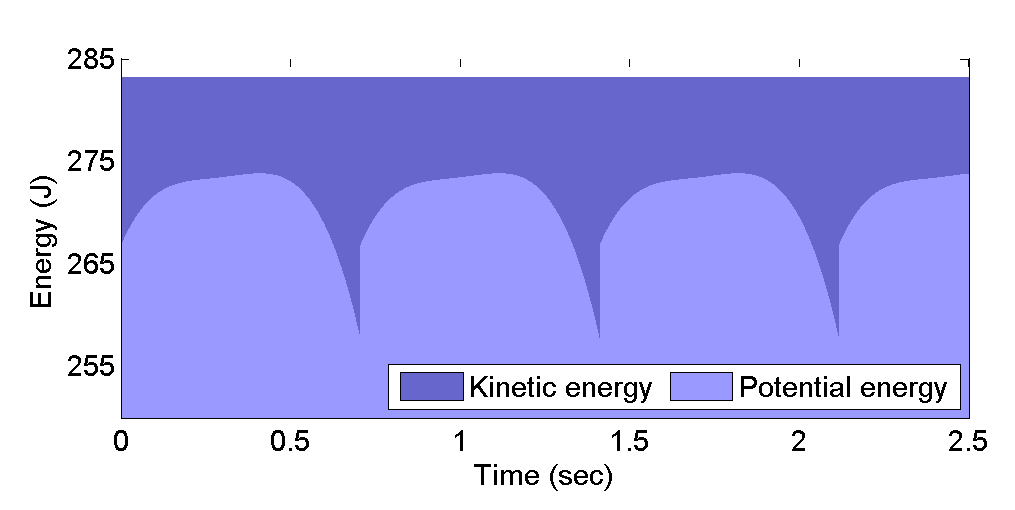
\includegraphics[width=1.0\columnwidth]{energy_cg2d_slope_model}
      \caption{Energy of the shaped system is conserved.}
    \end{figure}    
  }
  %  \only<3>{
  %    \includemedia[
  %      width=1.0\columnwidth,
  %      height=0.5625\columnwidth,
  %      addresource=amber2d.mp4,
  %      activate=pageopen,
  %      flashvars={source=amber2d.mp4&loop=true&autoPlay=true}
  %    ]{}{}%VPlayer9.swf}
  %  }

  \only<3>{
    Energy shaping can be achieved using:
    \begin{align}
      \nonumber
      \argmin_{v = (\delta, u)}  \, & v^T \! H \, v + h^T(q, \dot q) v\\
      \label{clf} \tag{clf}
      \mbox{s.t. } & \Aclf(q, \dot q) v \leq \bclf(q, \dot q)
    \end{align}
    where
    \begin{align*}
      H = \left(\begin{array}{c c}\epsilon & 0\\ 0 & I\end{array}\right), \qquad
        h(q, \dot q) = \left(\begin{array}{c} 0\\ -2 \, \bar u(q, \dot q) \end{array}\right),
    \end{align*}
    and
    \begin{align*}
      \Aclf = \left(\begin{array}{c c}
        -1 & 2 \eta L_{g} \eta
      \end{array}\right), \qquad
      \bclf = -\epsilon \eta^{2} - 2\eta L_{f} \eta
    \end{align*}
  }

  \only<4>{
    \begin{figure}
      \centering
      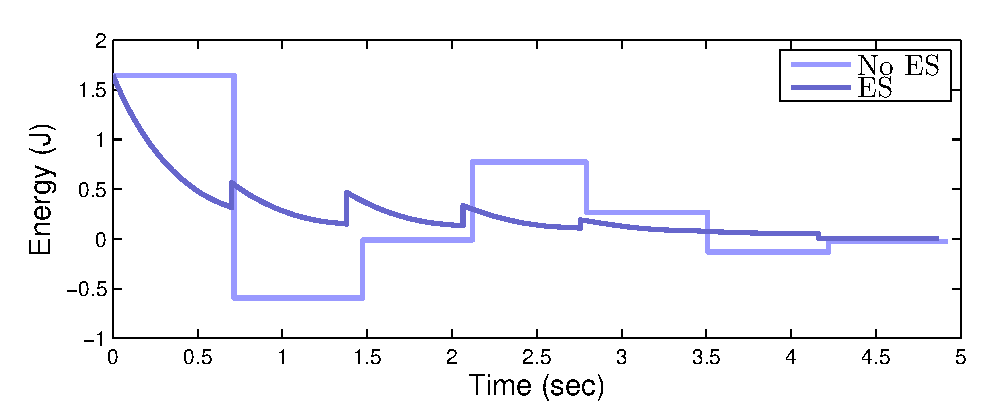
\includegraphics[width=1.0\columnwidth]{es_comparison_2link_conservative}
      \caption{Demonstration of energy shaping on 2-link biped.}
    \end{figure}
  }

  \only<5>{
    \begin{figure}
      \centering
      \includemedia[
        %width=1.0\columnwidth,
        %height=0.5625\columnwidth,
        width=1.0\columnwidth,
        height=0.5\columnwidth,
        addresource=cg2d_es.mp4,
        activate=pageopen,
        flashvars={source=cg2d_es.mp4&loop=true&autoPlay=true}
      ]{}{VPlayer9.swf}
      \caption{Energy shaping to stabilize to a gait from distant initial condition.}
    \end{figure}
  }

  \only<6> {
    \begin{figure}
      \centering
      \begin{subfigure}[t]{0.48\textwidth}
        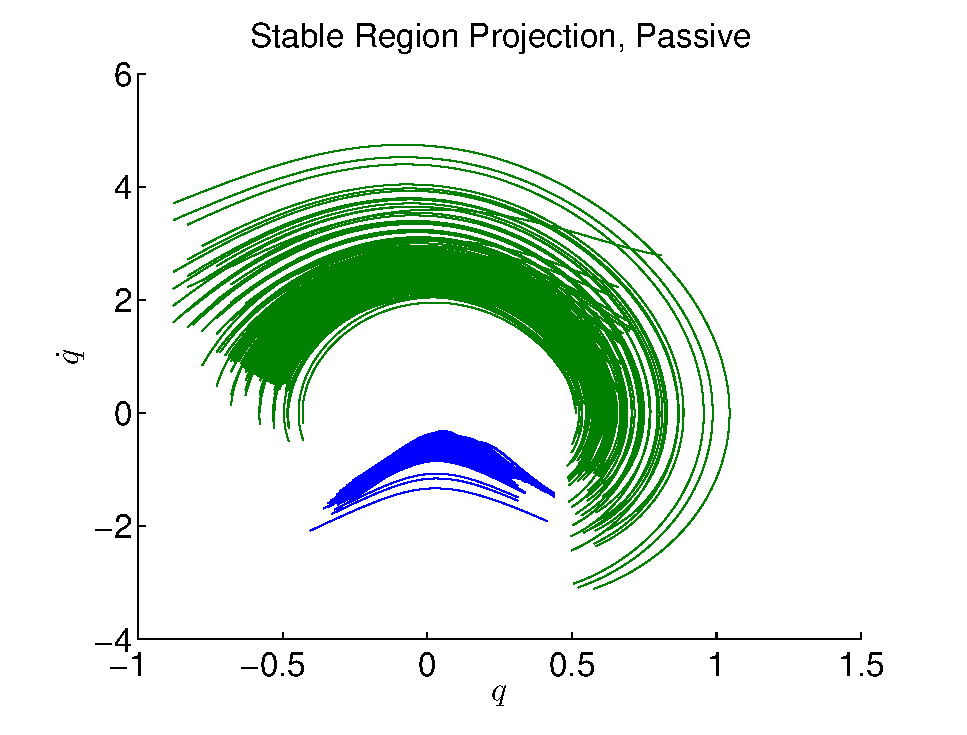
\includegraphics[width=\textwidth]{pp_eps_0}
        \caption{Nominal system.}
      \end{subfigure}%
      \hfill
      \begin{subfigure}[t]{0.48\textwidth}
        \includegraphics[width=\textwidth]{pp_eps_1_100}
        \caption{Shaped system with $\resclfparam = \frac{1}{100}$.}
      \end{subfigure}
      \caption{Comparison of unshaped and shaped system.}
    \end{figure}
  }

  \only<7> {
    \begin{figure}
      \centering
      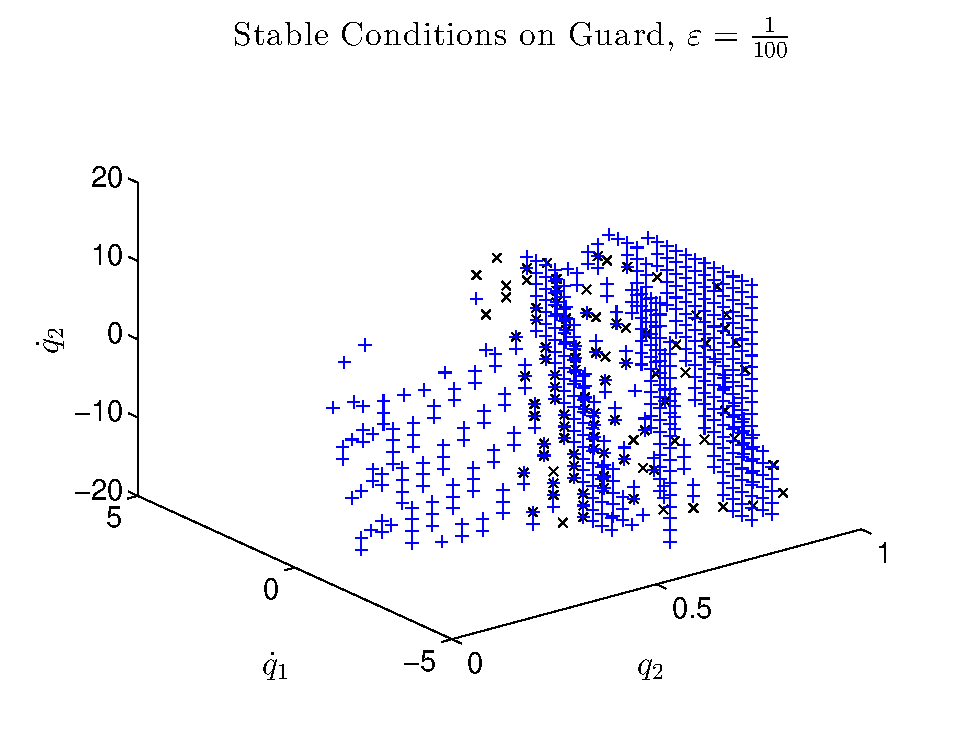
\includegraphics[height=.7\textheight]{poincare_cloud}
      \caption{A three-dimensional representation of the domain of attraction
        on the guard, comparing the unshaped and shaped system.}
    \end{figure}
  }
\end{frame}

\begin{frame}
  \frametitle{Example: 3-Link Biped}
  \only<1>{
    \begin{columns}
      \column{1.5in}
      Dynamic Model:
      \begin{align*}
        M(q) \ddot q + H(q, \dot q) = B(q) u
      \end{align*}
      Control Law:
      \begin{align*}
        {\bar u} &= G(q) - G(\Psi(q))\\
        {\bar u}_3 &=-k_{d} (\dot \vartheta_{T}^{a})\\
        &\hspace{1.8em} -k_{p} (\vartheta_{T}^{a} - \vartheta_{T}^{d})
      \end{align*}
      \column{1.5in}
      \begin{figure}
        \centering
        \def\svgwidth{1.0\columnwidth}
        \input{../figs/cg2d-3link-model.eps_latex}
        \vspace{-2em}
        \caption{3-link biped configuration.}
      \end{figure}
    \end{columns}
  }
  \only<2>{
    \begin{figure}
      \centering
      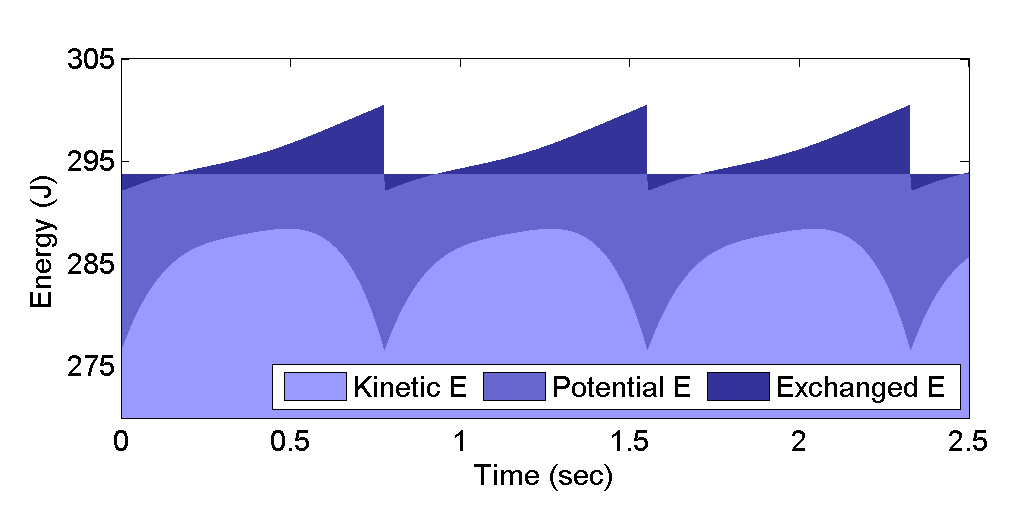
\includegraphics[width=1.0\columnwidth]{energy_conserved_cg2d_3link}
      \caption{The quantity, $E_{0}(\q, \dq) = T(\q, \dq) + V(\q) + \int_{t_{0}}^{t} F_{nc} \cdot \frac{d\q}{d\tau} d\tau$, is conserved.}
    \end{figure}
  }
  \only<3>{
    \begin{figure}
      \centering
      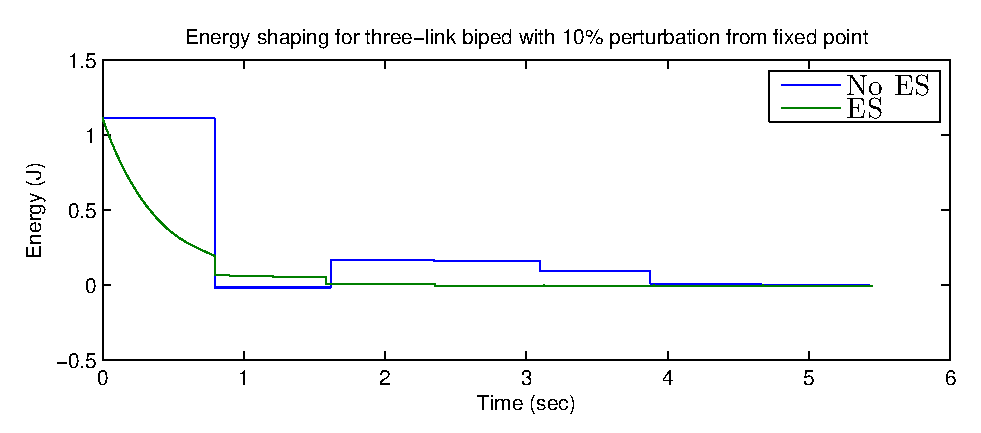
\includegraphics[width=1.0\columnwidth]{es_comparison_3link}
      \caption{Demonstration of energy shaping on 3-link biped.}
    \end{figure}
  }


  \only<4>{
    \begin{figure}
      \centering
      \includemedia[
        %width=1.0\columnwidth,
        %height=0.5625\columnwidth,
        width=1.0\columnwidth,
        height=0.5\columnwidth,
        addresource=3link_es.mp4,
        activate=pageopen,
        flashvars={source=3link_es.mp4&loop=true&autoPlay=true}
      ]{}{VPlayer9.swf}
      \caption{Energy shaping to stabilize to a gait from distant initial condition.}
    \end{figure}
  }

\end{frame}

\begin{frame}
  \frametitle{Multi-Domain Hybrid Systems}
  \begin{itemize}
  \item Complex hybrid systems are made by stitching together domains.
  \item Conserved energy is unique to each domain, i.e.,
    \begin{align*}
      E_0^{1} \to E_{0}^{2} \to \cdots \to E_{0}^{n-1} \to E_{0}^{n} \to E_{0}^{1} \to \cdots
    \end{align*}
  \item Each domain shapes to a specific conserved energy level.
  \end{itemize}
\end{frame}


\begin{frame}
  \frametitle{Example: 7-Link Biped with Feet}
  \only<1>{
    \blue{Appeared in {\bf Automatica}, Aug. 2014}
    \begin{columns}
      \column{1.5in}
      Dynamic Model:
      \begin{align*}
        M(q) \ddot q + H(q, \dot q) = J^{T}(q) \lambda + B(q) u
      \end{align*}
      \column{1.5in}
      \begin{figure}
        \centering
        \def\svgwidth{1.0\columnwidth}
        \input{../figs/cg2d-7link-model.eps_latex}
        \vspace{-2em}
        \caption{7-link biped configuration.}
      \end{figure}
    \end{columns}
  }

  \only<2>{
    \begin{block}{Spring--Damper Controller}
      \begin{align*}
        u(\q) = -\beta e^{-\rho \, h_{\mathrm{nst}}(\q)}
      \end{align*}
      where $\beta, \rho \in \R^{+}$ and $h_{\mathrm{nst}} : \ConfigurationSpace \to \R$ is the height of the Nonstance toe.
      Used on
      \begin{itemize}
      \item Stance ankle\\
      \item Nonstance ankle\\
      \item Absolute torso angle\\
      \item Non-stance knee spring (only in double support)
      \end{itemize}
      \blue{Provides passivity-based control and toe-off.}
    \end{block}
  }

  \only<3>{
    \begin{block}{Scuffing Prevention Controller}
      \begin{align*}
        u(\q) = k_p \theta(\q) - k_d \dot \theta(\dq)
      \end{align*}
      where $k_{p}, k_{d} \in \R^{+}$. Used on
      \begin{itemize}
      \item Nonstance ankle
      \end{itemize}
      \blue{Prevents the nonstance toe from colliding with the ground prematurely.}
    \end{block}
  }

\only<4>{
  \begin{figure}
    \centering
      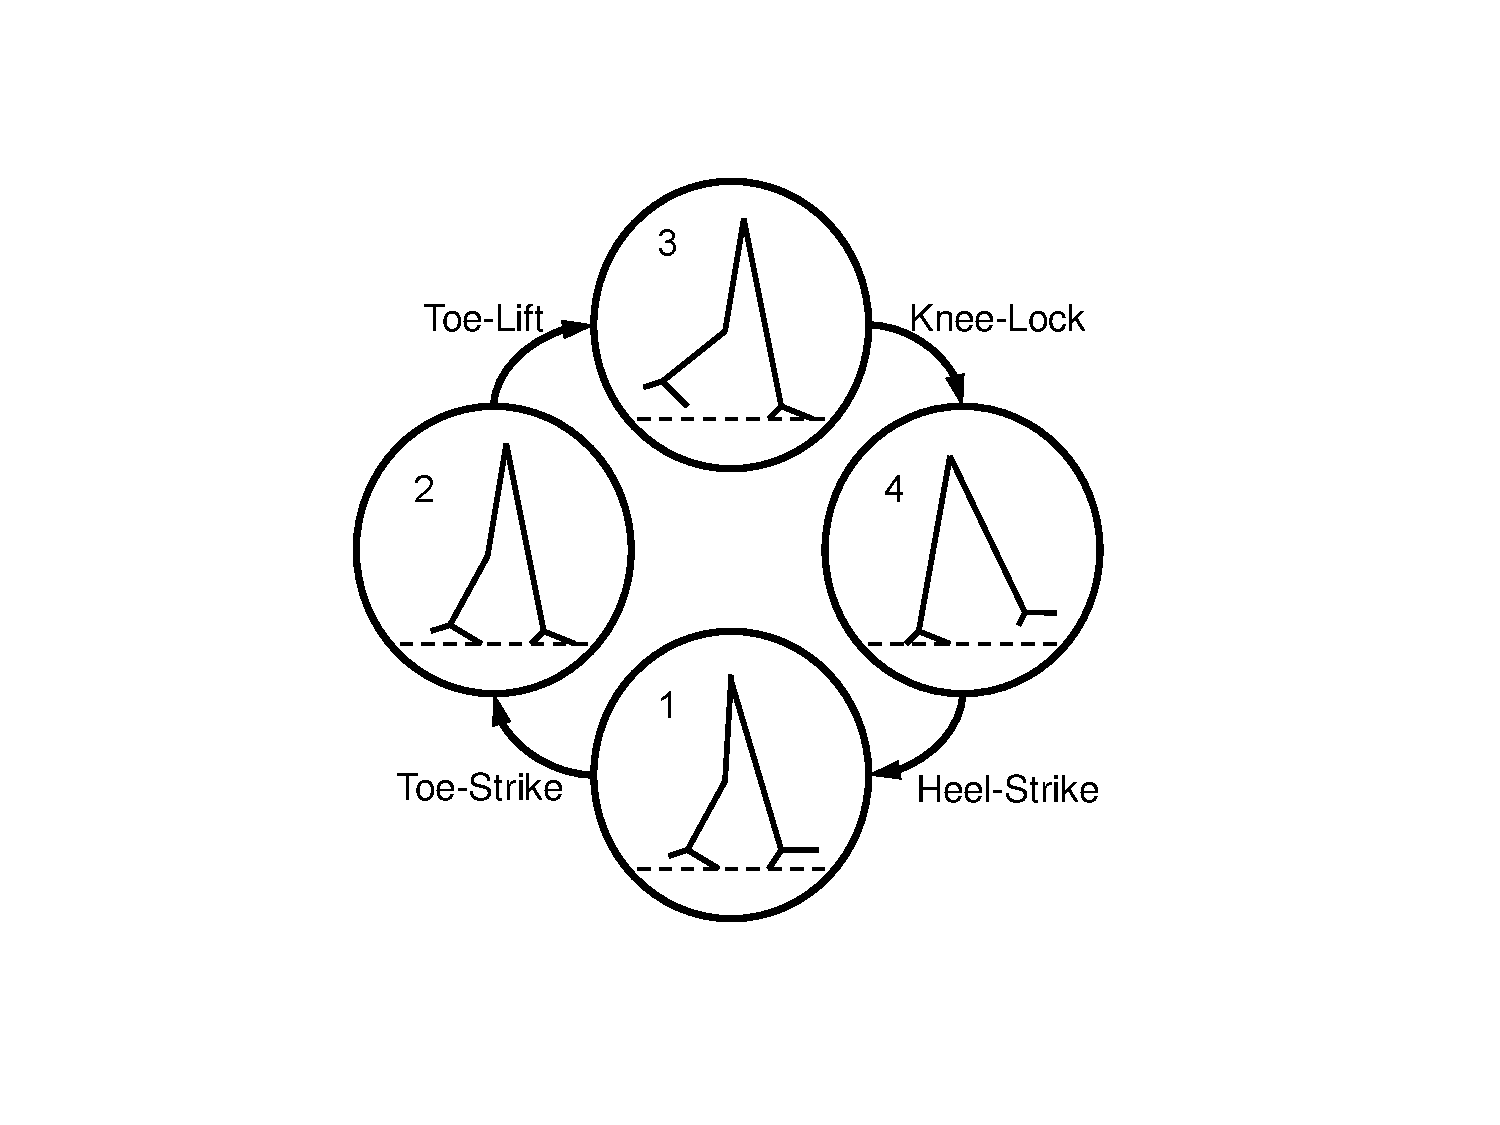
\includegraphics[height=.7\textheight]{domaingraph}
      \caption{The resulting gait traverses a four-domain directed graph.}
    \end{figure}
  }

  \only<5>{
    \begin{figure}
      \centering
      \includemedia[
        %width=1.0\columnwidth,
        %height=0.5625\columnwidth,
        width=1.0\columnwidth,
        height=0.5\columnwidth,
        addresource=7link_es.mp4,
        activate=pageopen,
        flashvars={source=7link_es.mp4&loop=true&autoPlay=true}
      ]{}{VPlayer9.swf}
      \caption{Energy shaping to stabilize to a gait.}
    \end{figure}
  }

  \only<6>{
    \begin{figure}
      \centering
      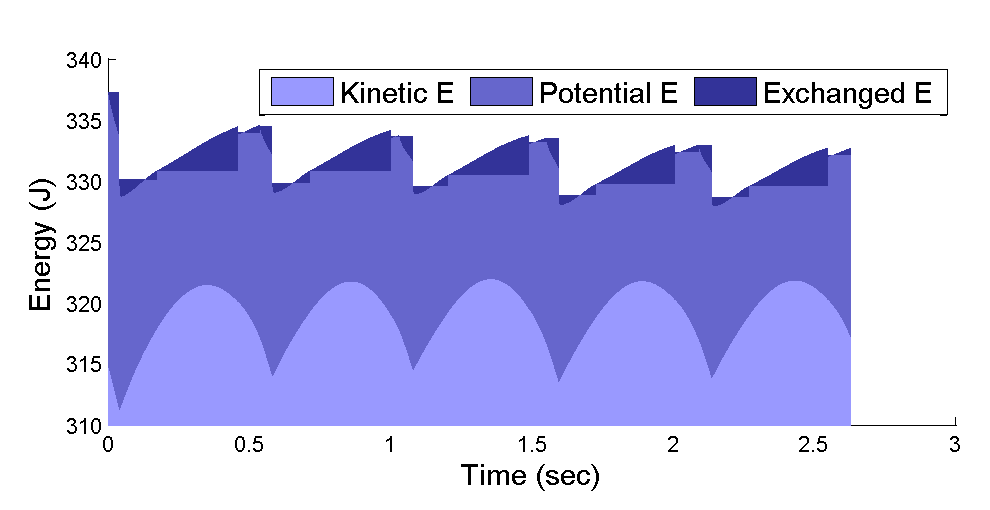
\includegraphics[width=1.0\columnwidth]{energy_conserved_7link}
      \caption{The quantity, $E_{0} \equiv T(q, \dot q) + V(q) + \int_{t_0}^{t} F_{nc} \cdot \frac{d\q}{d\tau} d\tau$, is conserved.}
    \end{figure}
  }

  \only<7>{
    \begin{figure}
      \centering
      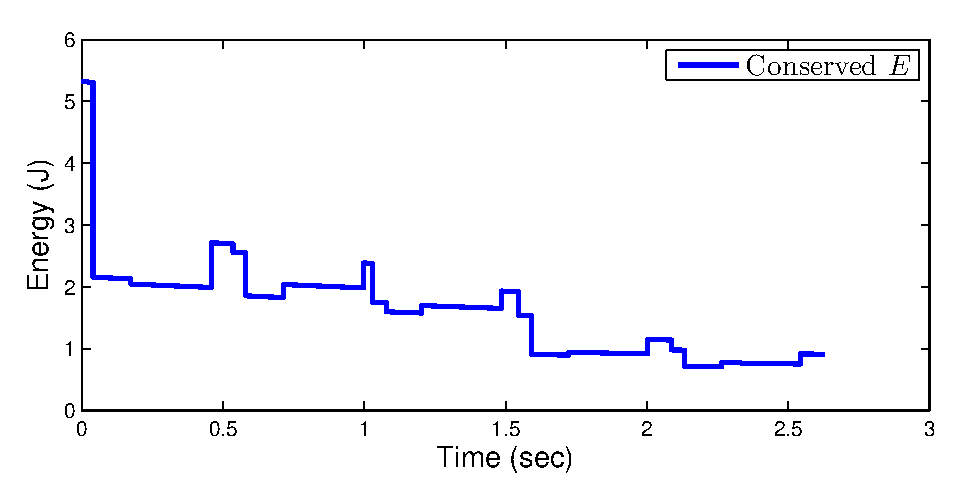
\includegraphics[width=1.0\columnwidth]{energy_conserved_7link_outline}
      \caption{The quantity, $E_{0} \equiv T(q, \dot q) + V(q) + \int_{t_0}^{t} F_{nc} \cdot \frac{d\q}{d\tau} d\tau$, is conserved.}
    \end{figure}
  }
  \only<8>{
    \begin{figure}
      \centering
      \includemedia[
        %width=1.0\columnwidth,
        %height=0.5625\columnwidth,
        width=1.0\columnwidth,
        height=0.5\columnwidth,
        addresource=7link_noes.mp4,
        activate=pageopen,
        flashvars={source=7link_noes.mp4&loop=true&autoPlay=true}
      ]{}{VPlayer9.swf}
      \caption{Many steps on the limit cycle.}
    \end{figure}
  }
\end{frame}
